\documentclass{beamer}
\setbeamertemplate{frametitle}[default][center]
%Information to be included in the title page:
\title{\Large\textbf{Dydaktyczny symulator wybranych rozwiązań warstwy fizycznej sieci Ethernet}}
\author{Michał Iwanicki, Mateusz Bauer, Marcin Garnowski}
\institute{Politechnika Gdańska}
\date{2023}

\begin{document}

\frame{\titlepage}

\begin{frame}
\frametitle{Uruchamianie}

\includegraphics[width=0.25\textwidth]{images/prezentacja_start1.png}
\hfill
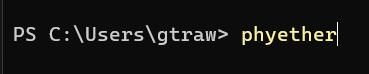
\includegraphics[width=0.65\textwidth]{images/prezentacja_start2.png}
\end{frame}

\begin{frame}
\frametitle{Poruszanie się po symulatorze}

\includegraphics[width=0.95\textwidth]{images/zakladki.png}
\end{frame}

\begin{frame}
\frametitle{Reed-Solomon}
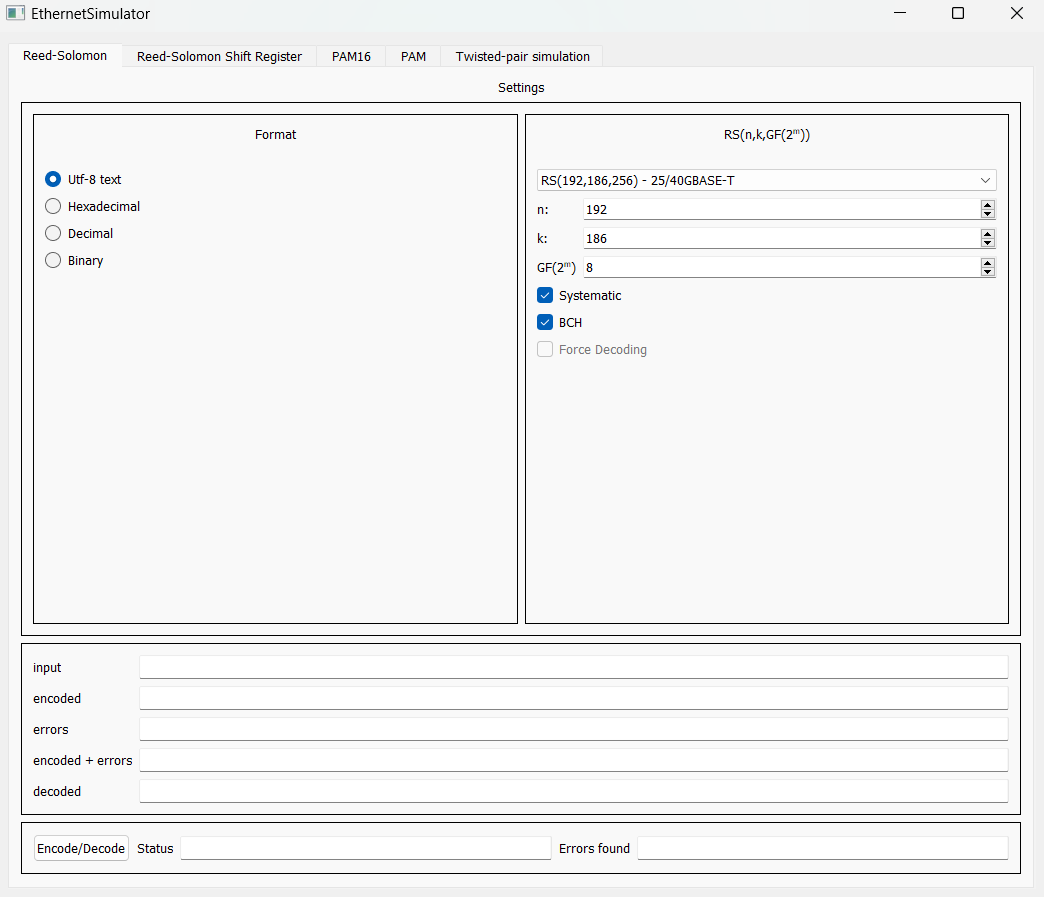
\includegraphics[width=0.95\textwidth]{images/prezentacja_rs.png}
\end{frame}

\begin{frame}
\frametitle{Reed-Solomon Shift Register}
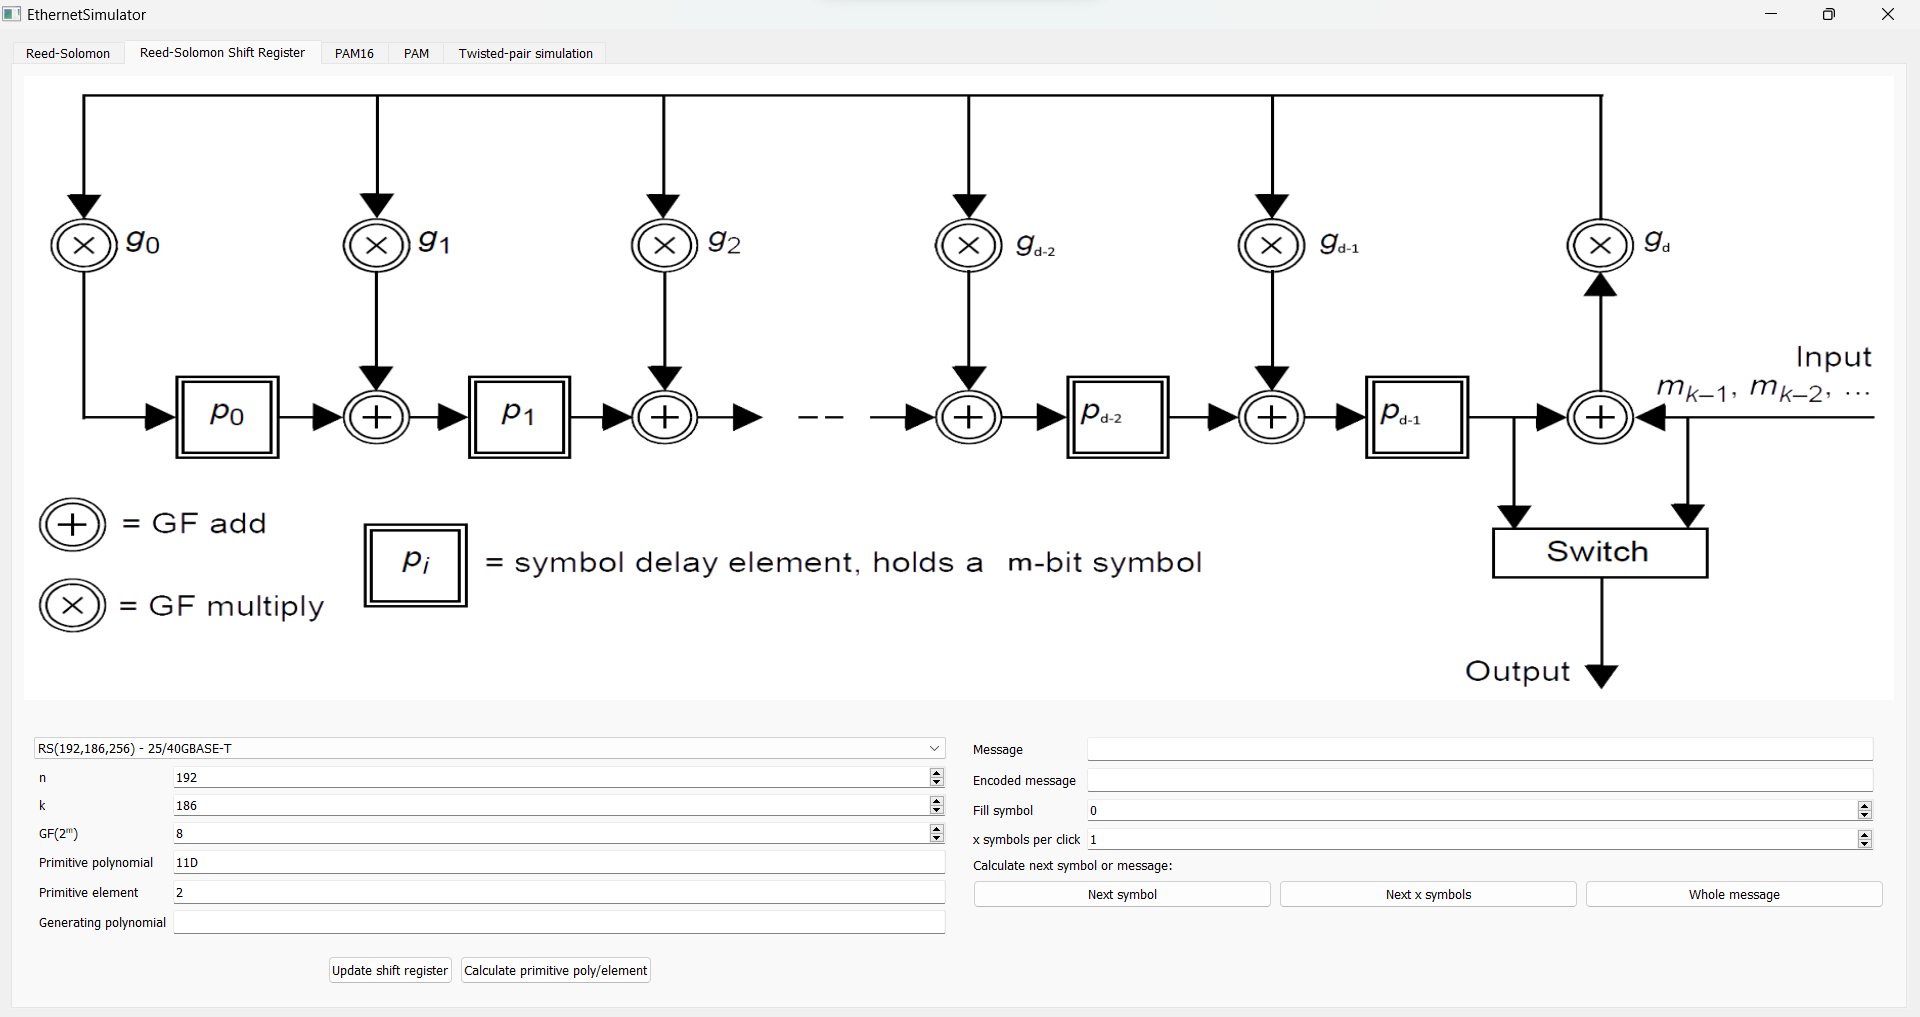
\includegraphics[width=0.95\textwidth]{images/prezentacja_rs_sr.png}
\end{frame}

\begin{frame}
\frametitle{PAM16}
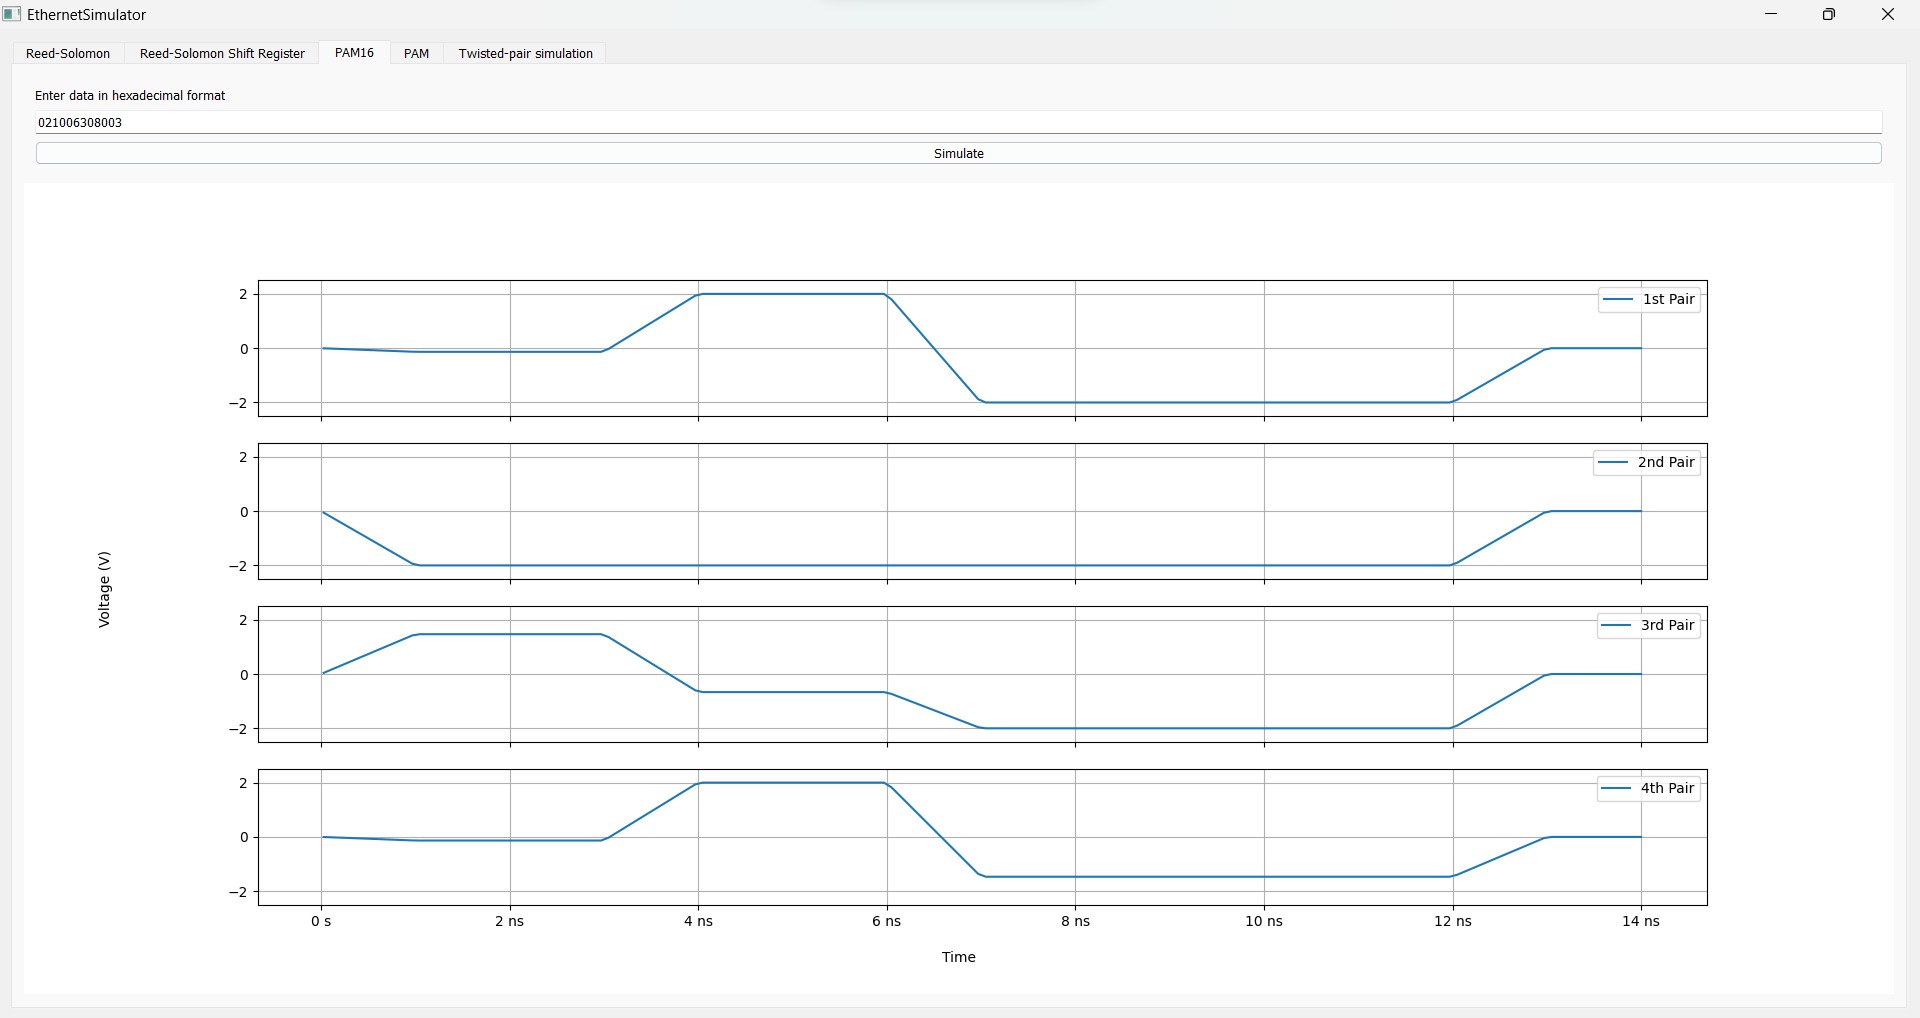
\includegraphics[width=0.95\textwidth]{images/prezentacja_pam16.png}
\end{frame}

\begin{frame}
\frametitle{PAM}
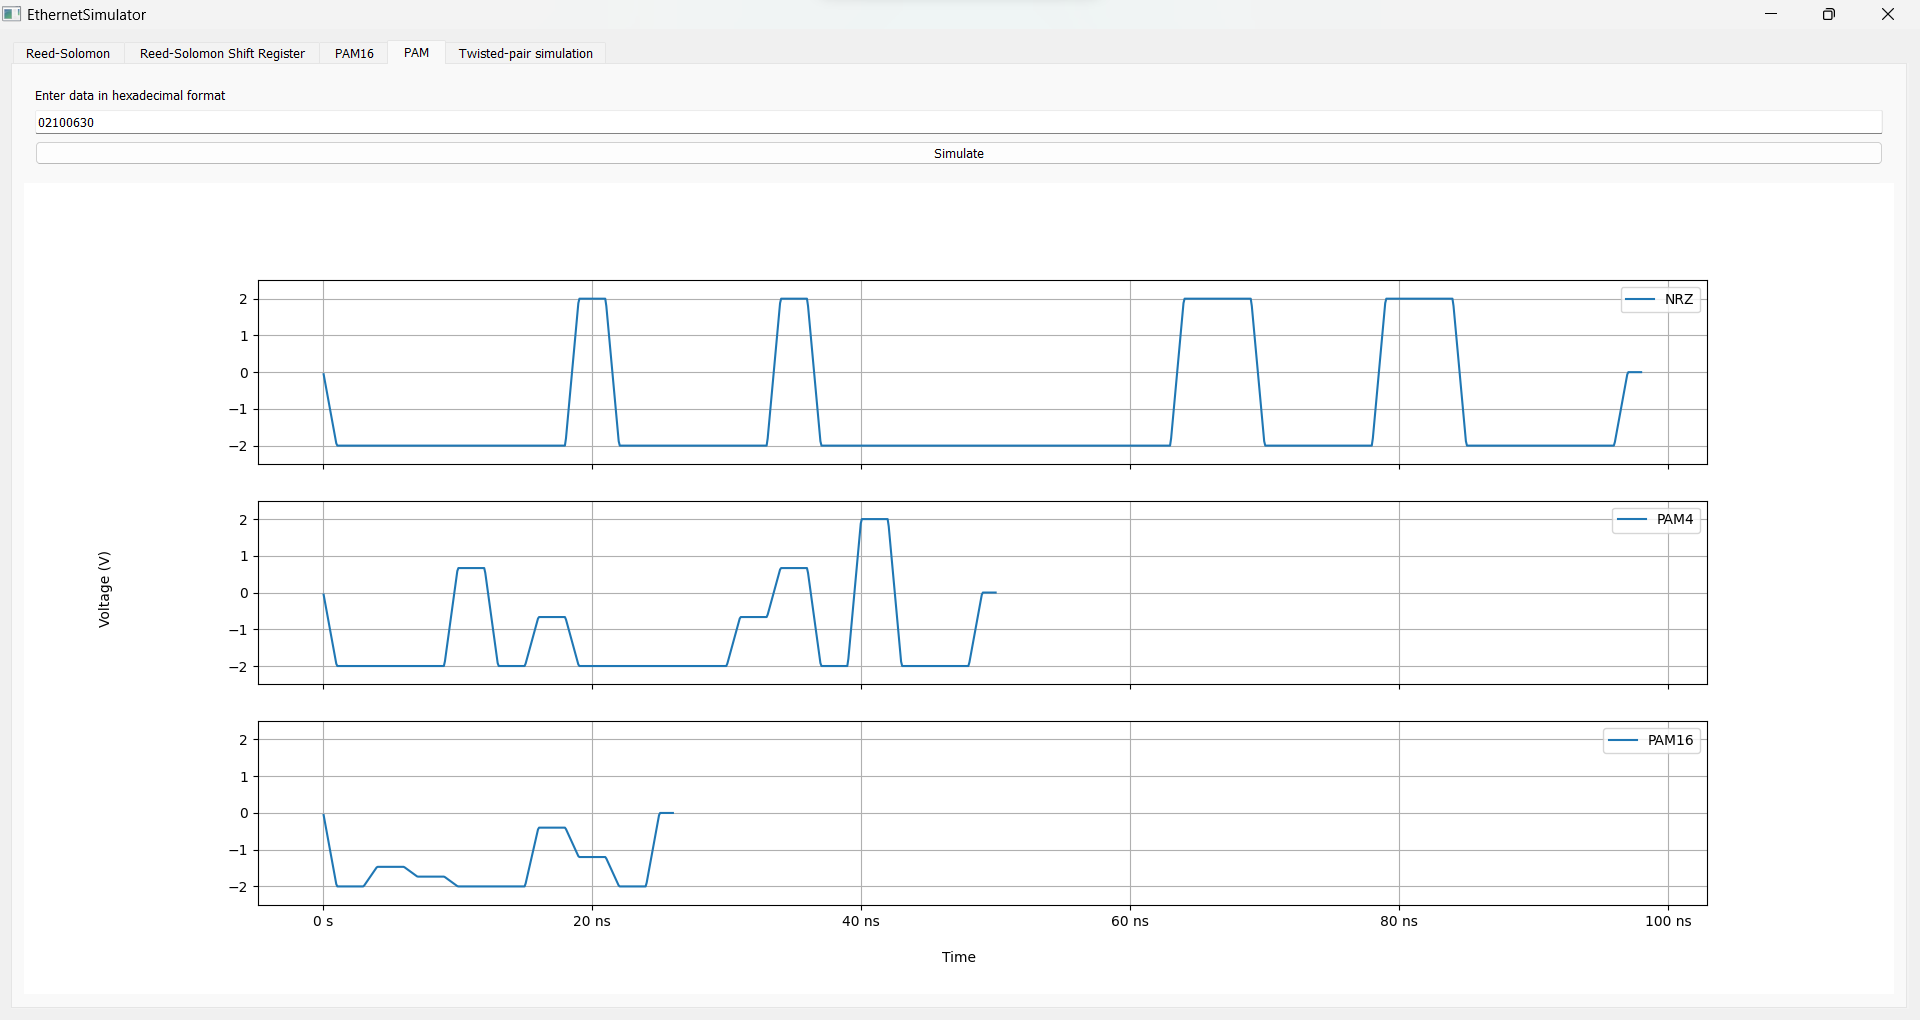
\includegraphics[width=0.95\textwidth]{images/prezentacja_pam.png}
\end{frame}

\begin{frame}
\frametitle{Twisted-pair simulation}
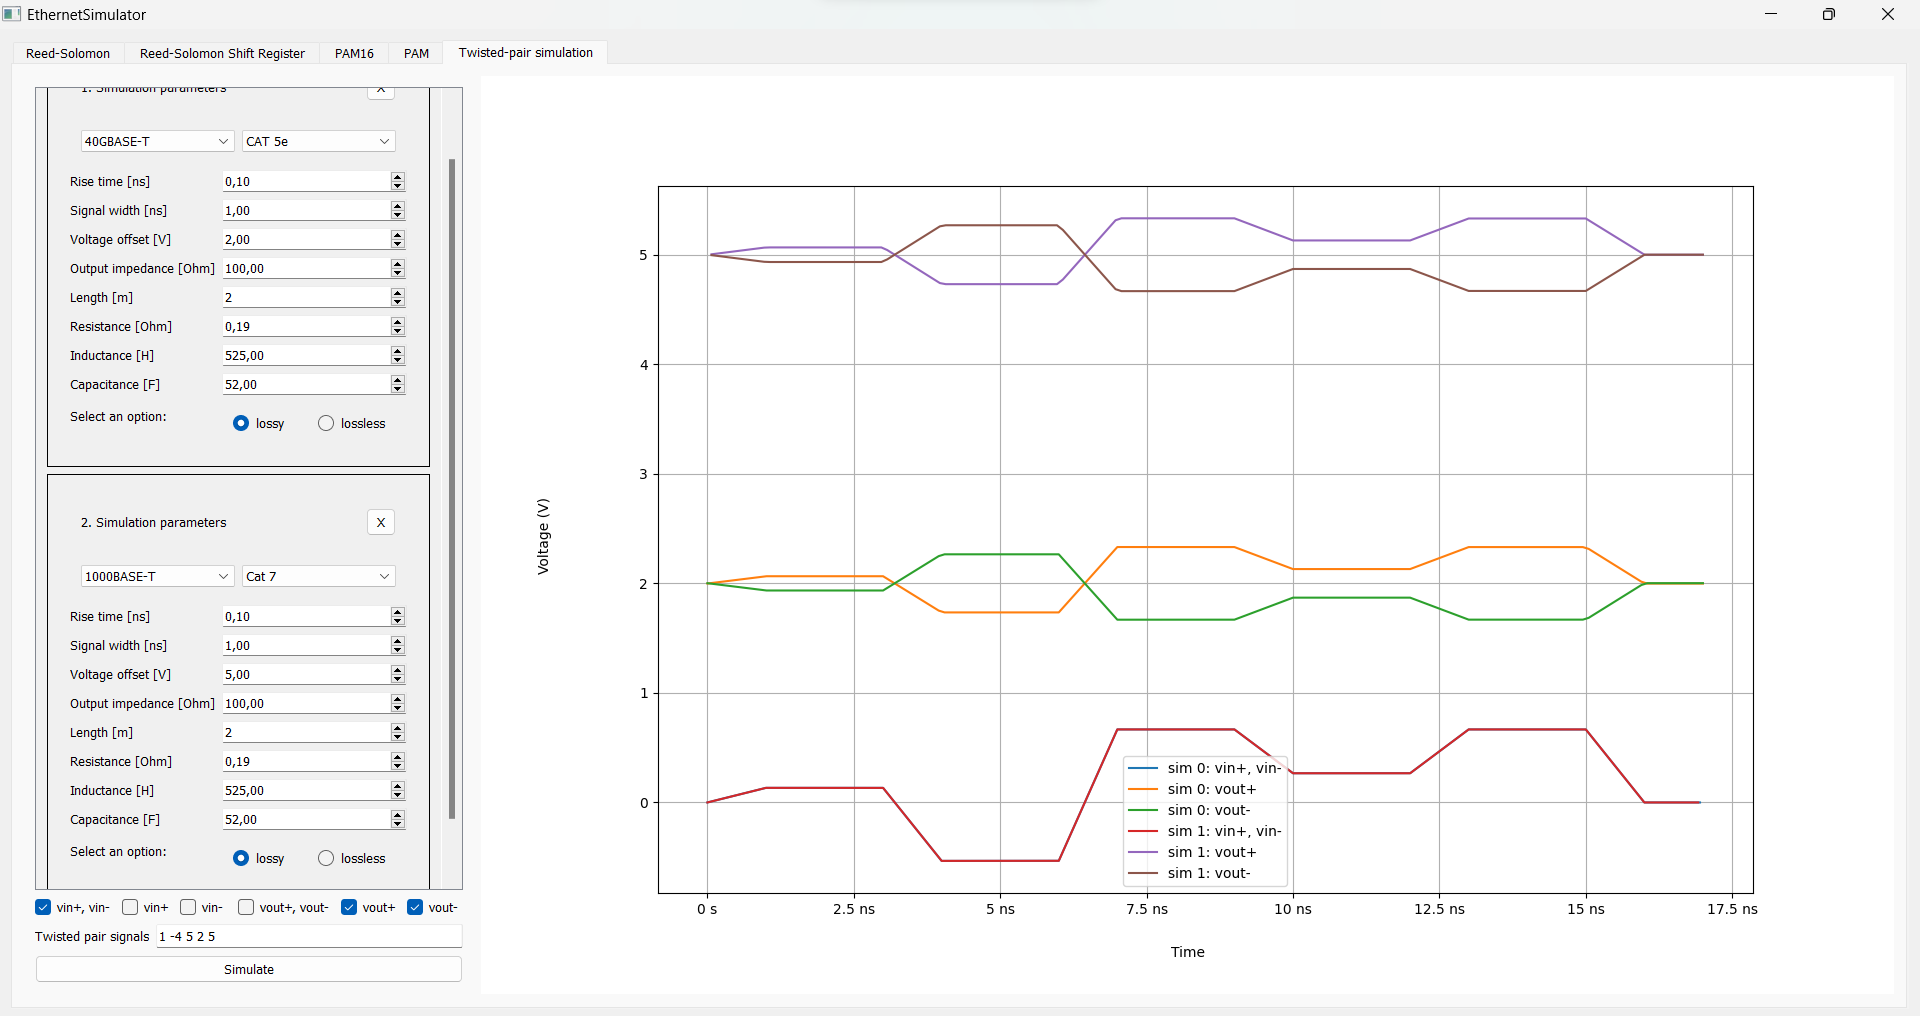
\includegraphics[width=0.95\textwidth]{images/prezentacja_tp.png}
\end{frame}

\begin{frame}
\frametitle{Modulacja}
Modulacja cyfrowa --- technika zamiany bitów na sygnał oraz sygnału na bity
\end{frame}

\begin{frame}
\frametitle{PAM}
\begin{enumerate}
    \item Pulse-Amplitude Modulation --- jedna z najpopularniejszych technik modulacji (Ethernet, USB4, PCI Express 6.0)
    \item Dane przesyłane jako zmiany amplitudy sygnału
    \item PAM-N --- N oznacza liczbę wykorzystywanych poziomów
\end{enumerate}
\end{frame}

\begin{frame}
\frametitle{NRZ (PAM2)}
\begin{itemize}
    \item 1 symbol koduje 1 bit
\end{itemize}
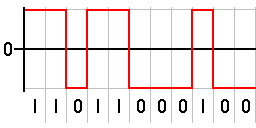
\includegraphics[width=0.95\textwidth]{images/nrz_code.png}
\end{frame}

\begin{frame}
\frametitle{NRZ (PAM2)}
Chcemy mieć większą przepustowość --- czy inny sposób modulacji może nam w tym pomóc?
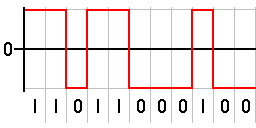
\includegraphics[width=0.95\textwidth]{images/nrz_code.png}
\end{frame}

\begin{frame}
\frametitle{PAM4}
\begin{itemize}
    \item 1 symbol koduje 2 bity
\end{itemize}
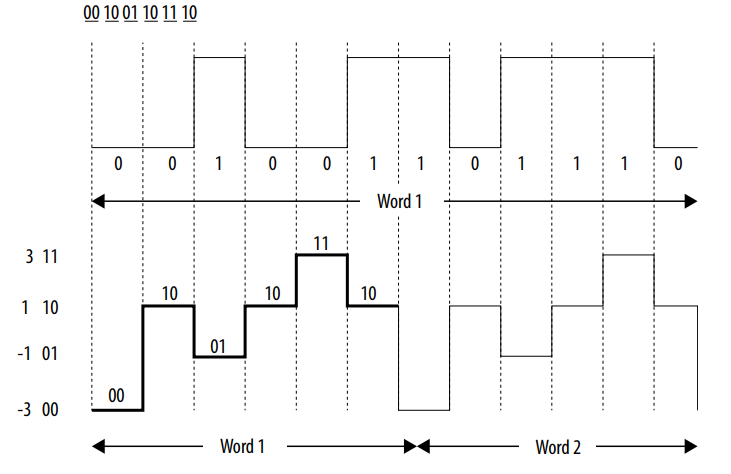
\includegraphics[width=0.95\textwidth]{images/pam4_vs_nrz.png}
\end{frame}

\begin{frame}
\frametitle{PAM4}
Plusy:
\begin{enumerate}
    \item 2x większa przepustowość bez zwiększania szerokości pasma (++)
\end{enumerate}

Minusy:
\begin{enumerate}
    \item 6 narastających zbocz, 6 opadających zbocz --- w sumie 12 zmian napięcia --- spada stosunek sygnału do szumu (SNR)
    \item Różnica pomiędzy przesyłanymi symbolami maleje --- potrzebujemy lepszego sprzętu do odczytu i intepretacji sygnału
\end{enumerate}
\end{frame}

\begin{frame}
\frametitle{PAM4}
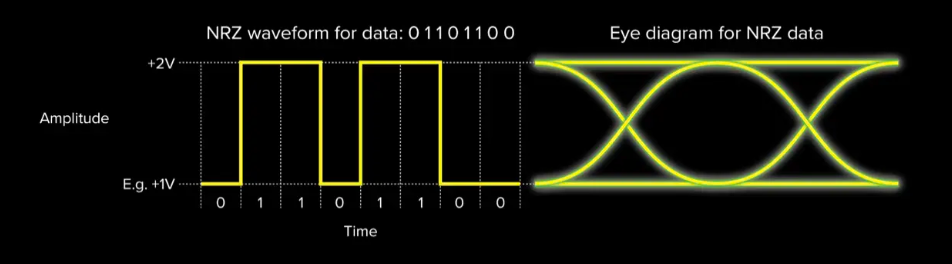
\includegraphics[width=0.95\textwidth]{images/eye_diagram_nrz.png}
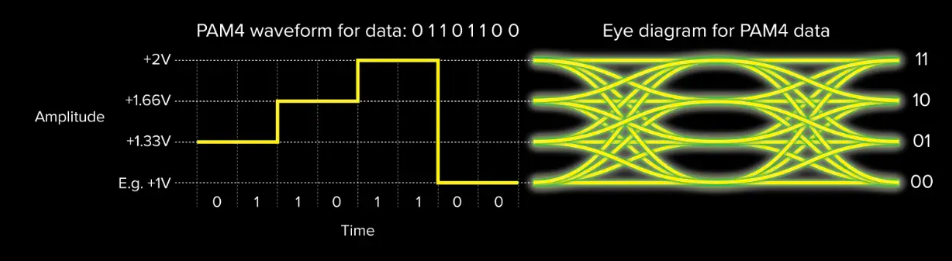
\includegraphics[width=0.95\textwidth]{images/eye_diagram_pam4.png}
100GbE, 200GbE, 400GbE
\end{frame}

\begin{frame}
\frametitle{PAM16}
\begin{itemize}
    \item 1 symbol koduje 4 bity
\end{itemize}
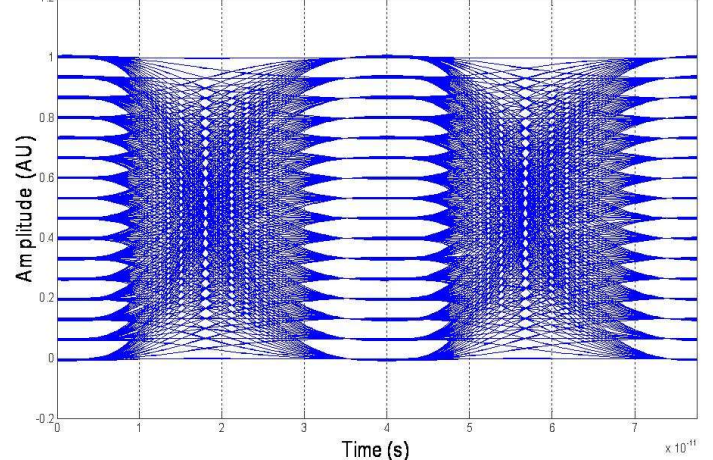
\includegraphics[width=0.95\textwidth]{images/eye_diagram_pam16.png}
\end{frame}

\begin{frame}
\frametitle{PAM - porównanie}
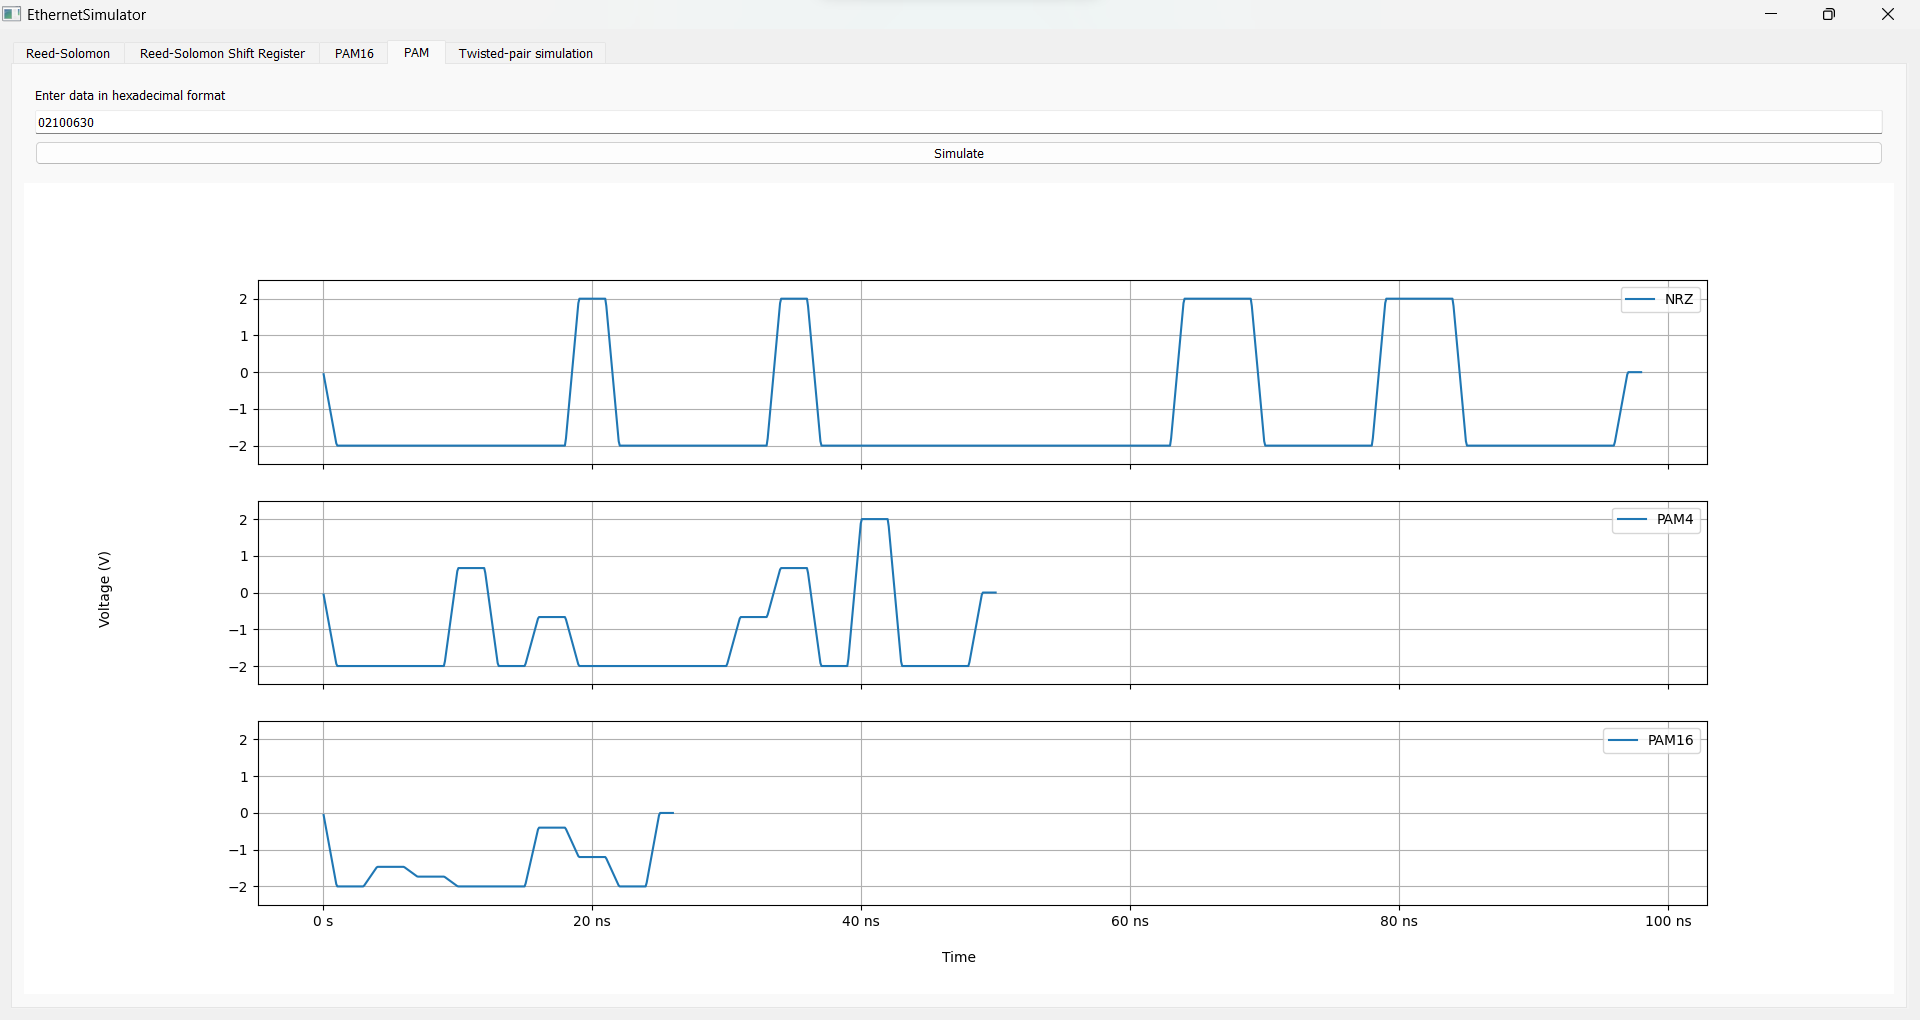
\includegraphics[width=0.95\textwidth]{images/prezentacja_pam.png}
\end{frame}

\begin{frame}
\frametitle{PAM - porównanie}
\begin{table}[h]
\centering
    \begin{tabular}{m{3cm} m{3cm} m{3cm}}
    \toprule
    Standard & Medium & Modulacja \\
    \midrule
    10GBASE-T & skrętka & PAM16 \\
    \midrule
    10GBASE-SR & światłowód & NRZ \\
    \midrule
    25GBASE-T & skrętka & PAM16 \\
    \midrule
    25GBASE-SR & światłowód & NRZ \\
    \midrule
    40GBASE-T & skrętka & PAM16 \\
    \midrule
    50GBASE-SR & światłowód & PAM4 \\
    \midrule
    100GBASE-ZR & światłowód & PAM4 \\
    \midrule
    200GBASE-SR2 & światłowód & PAM4 \\
    \midrule
    400GBASE-SR4 & światłowód & PAM4 \\
    \bottomrule
    \end{tabular}
\end{table}
\end{frame}

\end{document}